\section{Uncertainties in $\chi(k)$}
\begin{frame}\frametitle{Propagation of uncertainties in $\chi(k)$}

\begin{cenpage}{95mm}

  Estimating uncertainties in  $\chi(k)$ has always been a challenge.

  \vmm

  We have (by default) estimated the uncertainty in $\chi(k)$ as
  {\BlueEmph{white noise}} {\tiny{(Newville, Boyanov, and Sayers, {\emph{J
          Synch Rad}}, 1999)}}, using $\chi(R)$ between [15, 25] \AA.

\end{cenpage}

\begin{columns}
  \begin{column}[T]{60mm}

    {\onslide+<1->  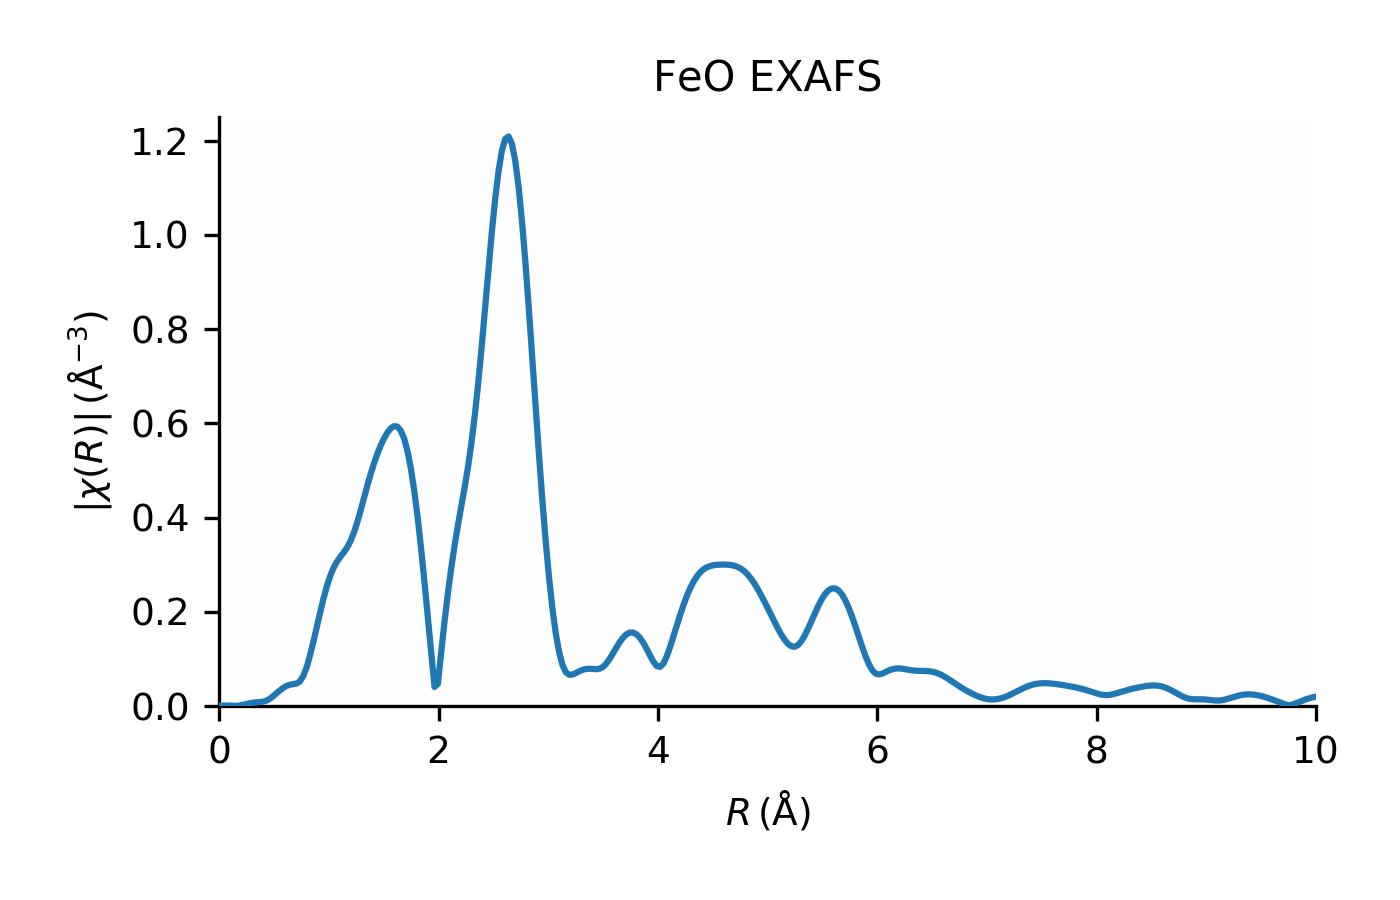
\includegraphics[width=60mm]{figs/errors/feo_chir}  }


  \end{column}
  \begin{column}[T]{60mm}

    {\onslide+<2-> 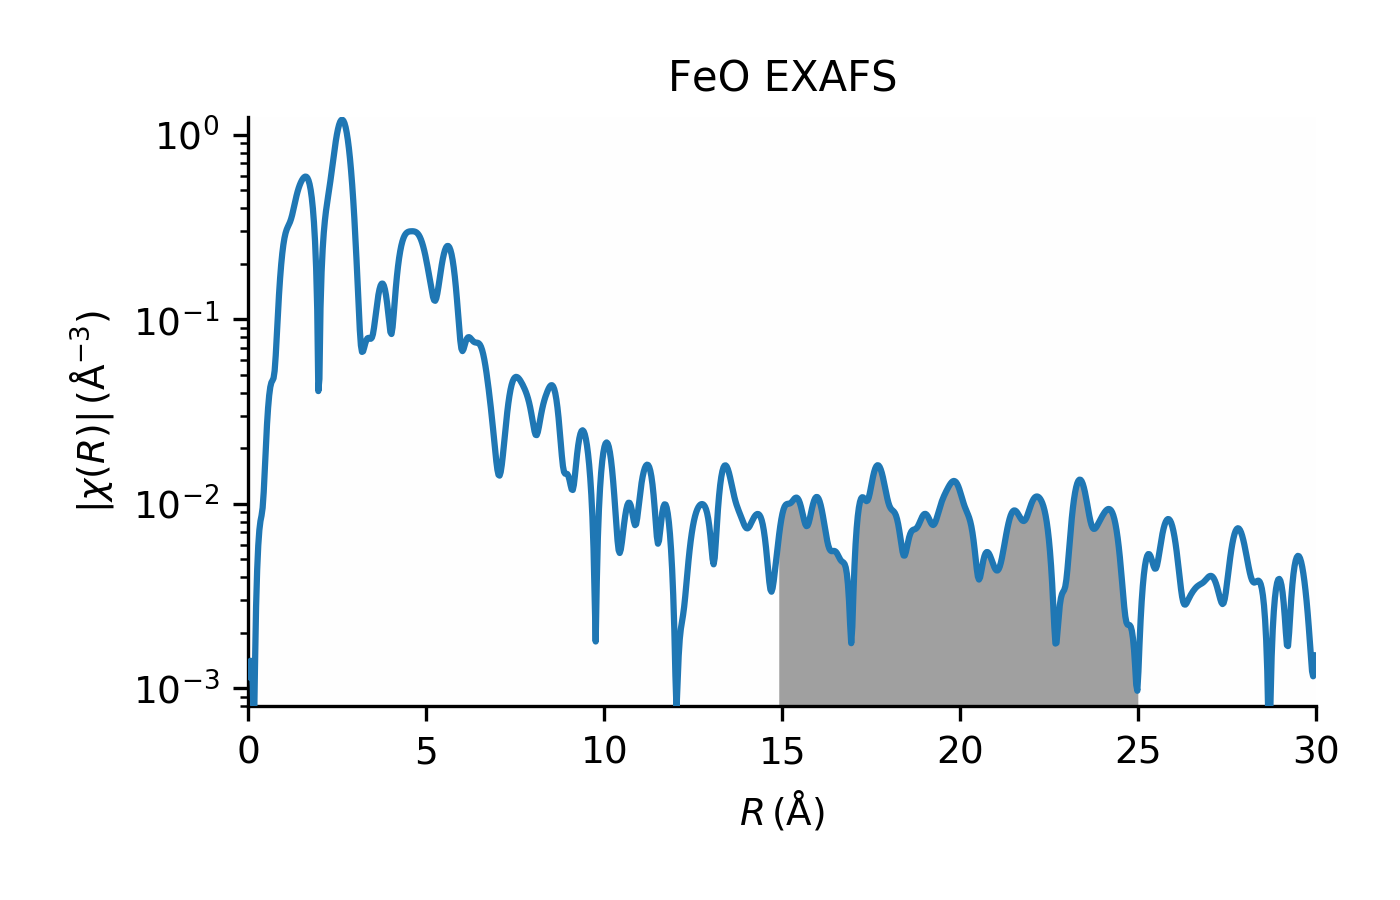
\includegraphics[width=60mm]{figs/errors/feo_chir_logscale} }

  \end{column}
\end{columns}

{\onslide+<3->

  \begin{cenpage}{105mm}


    The ``high-R'' portion of $\chi(R)$ can estimate the
    ``white noise'' in the data pretty well.

    \vmm
    This is easy to do, but we know it misses an important component:
  \end{cenpage}


  \begin{postitbox}{53mm}
      \RedEmph{uncertainties from  background subtraction}
  \end{postitbox}

}

\end{frame}


\begin{frame}\frametitle{ Uncertainties in $\chi(k)$ from background subtraction}


\vmm
\begin{cenpage}{105mm}

  We can propagate the uncertainties from the fit of the background spline
  to estimate the uncertainty in $\chi(k)$ from the background subtraction.

  \vmm \vmm

  This is {\BlueEmph{not white noise}}.   In fact, it tends to have a peak
  somewhat above $2 R_{\rm bkg}$
\end{cenpage}

\begin{columns}
  \begin{column}[T]{60mm}

    {\only<1> { 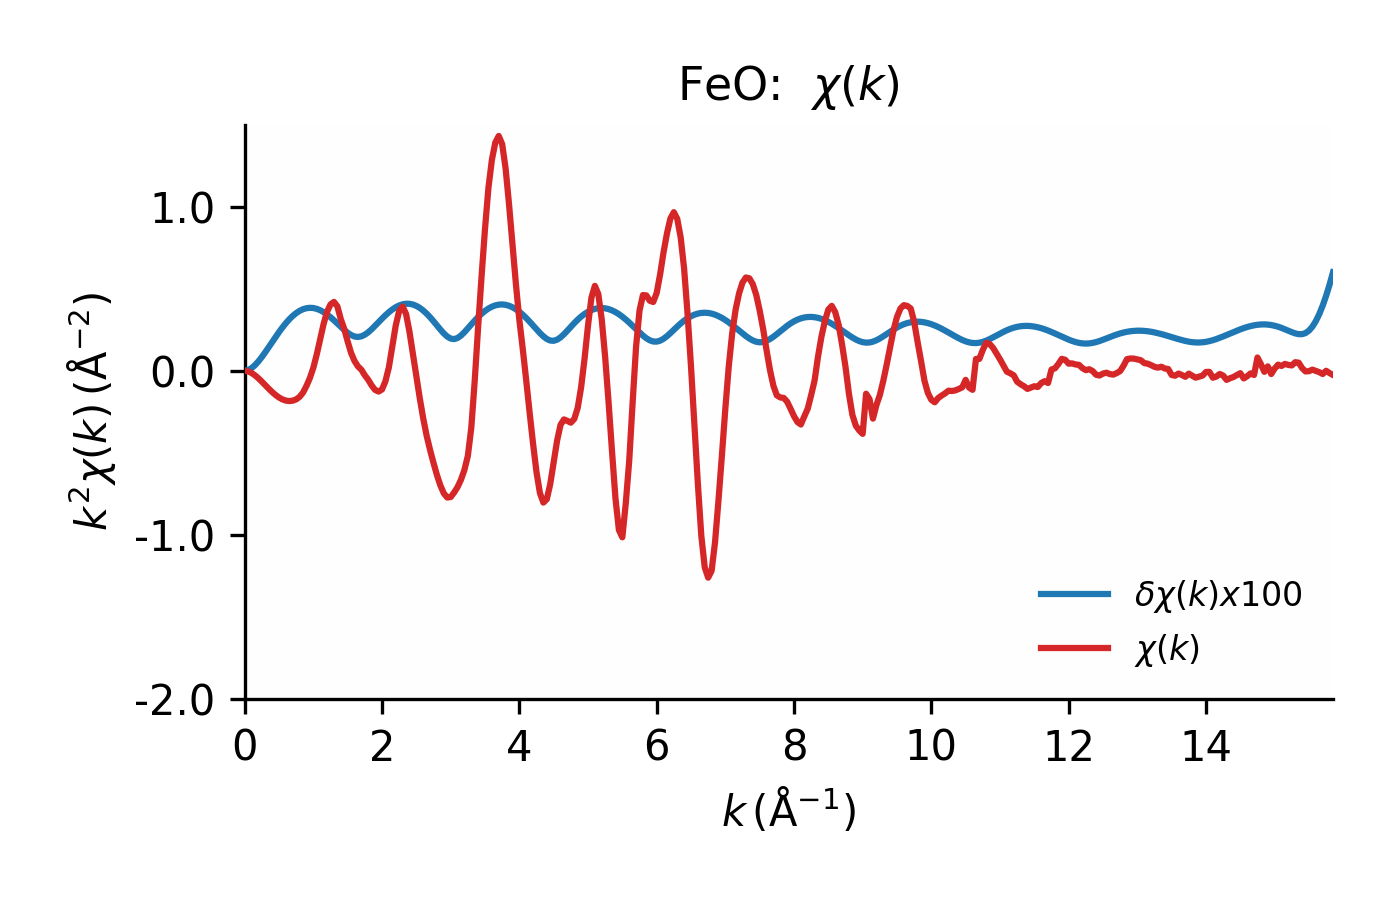
\includegraphics[width=60mm]{figs/errors/feo_chik_deltachi}}}

    {\only<2,3> { 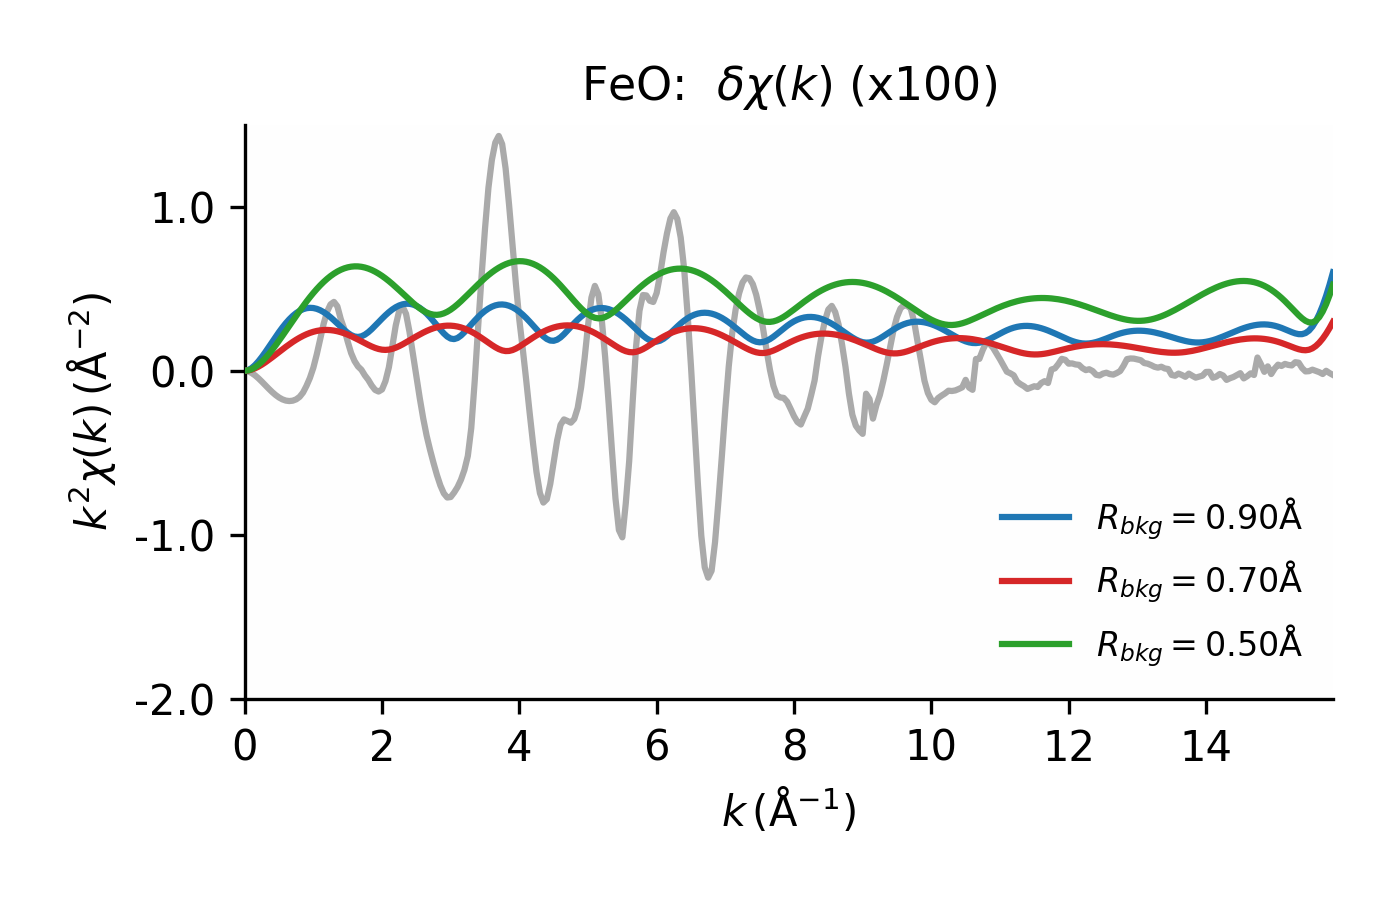
\includegraphics[width=60mm]{figs/errors/feo_deltachik_rbkg} }}

    \end{column}

    \begin{column}[T]{60mm}

      {\only<1>{ 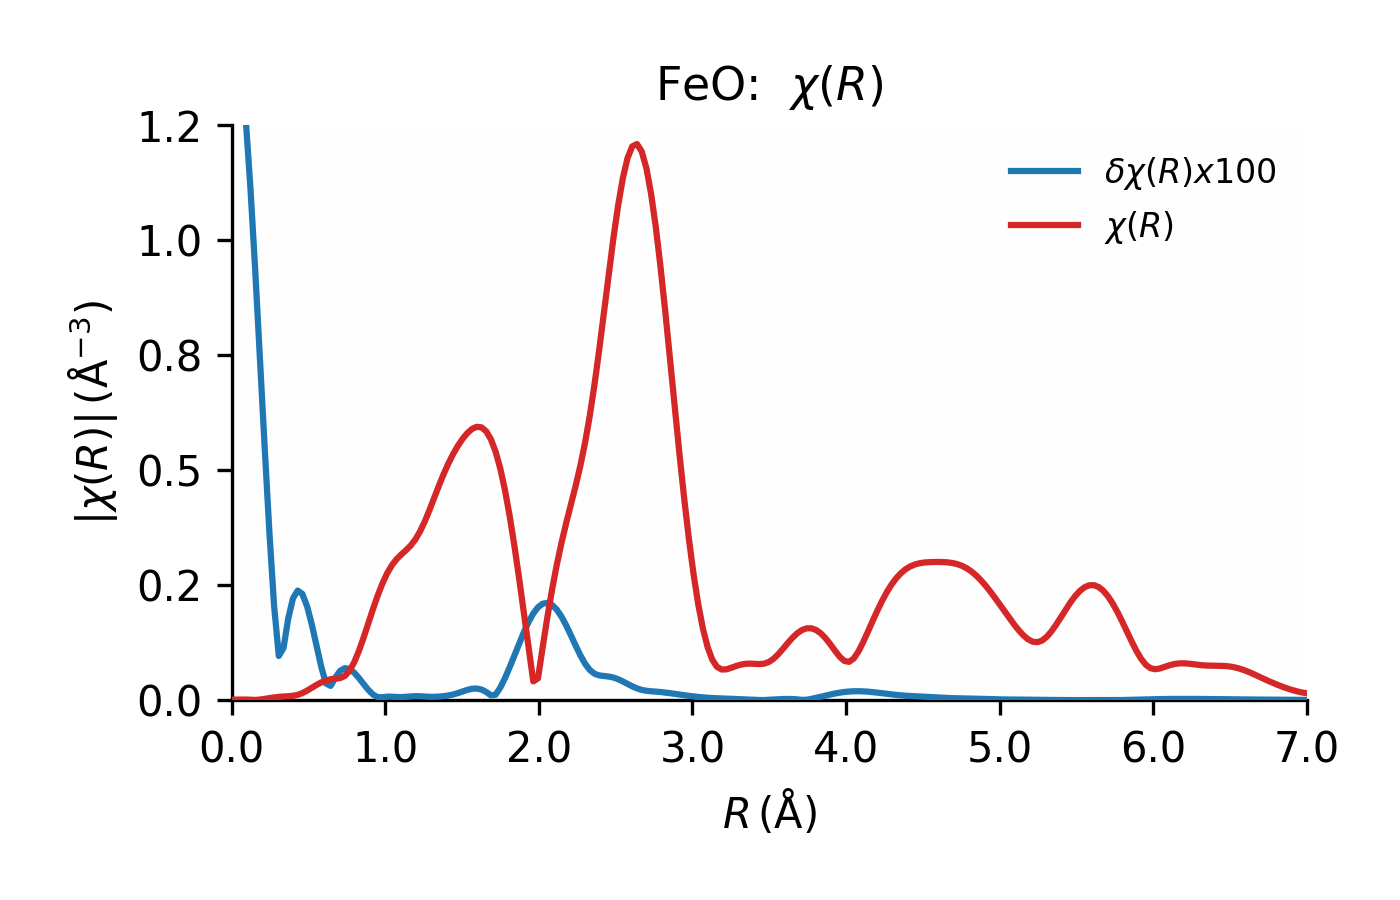
\includegraphics[width=60mm]{figs/errors/feo_chir_deltachi} }}
      {\only<2,3>{ 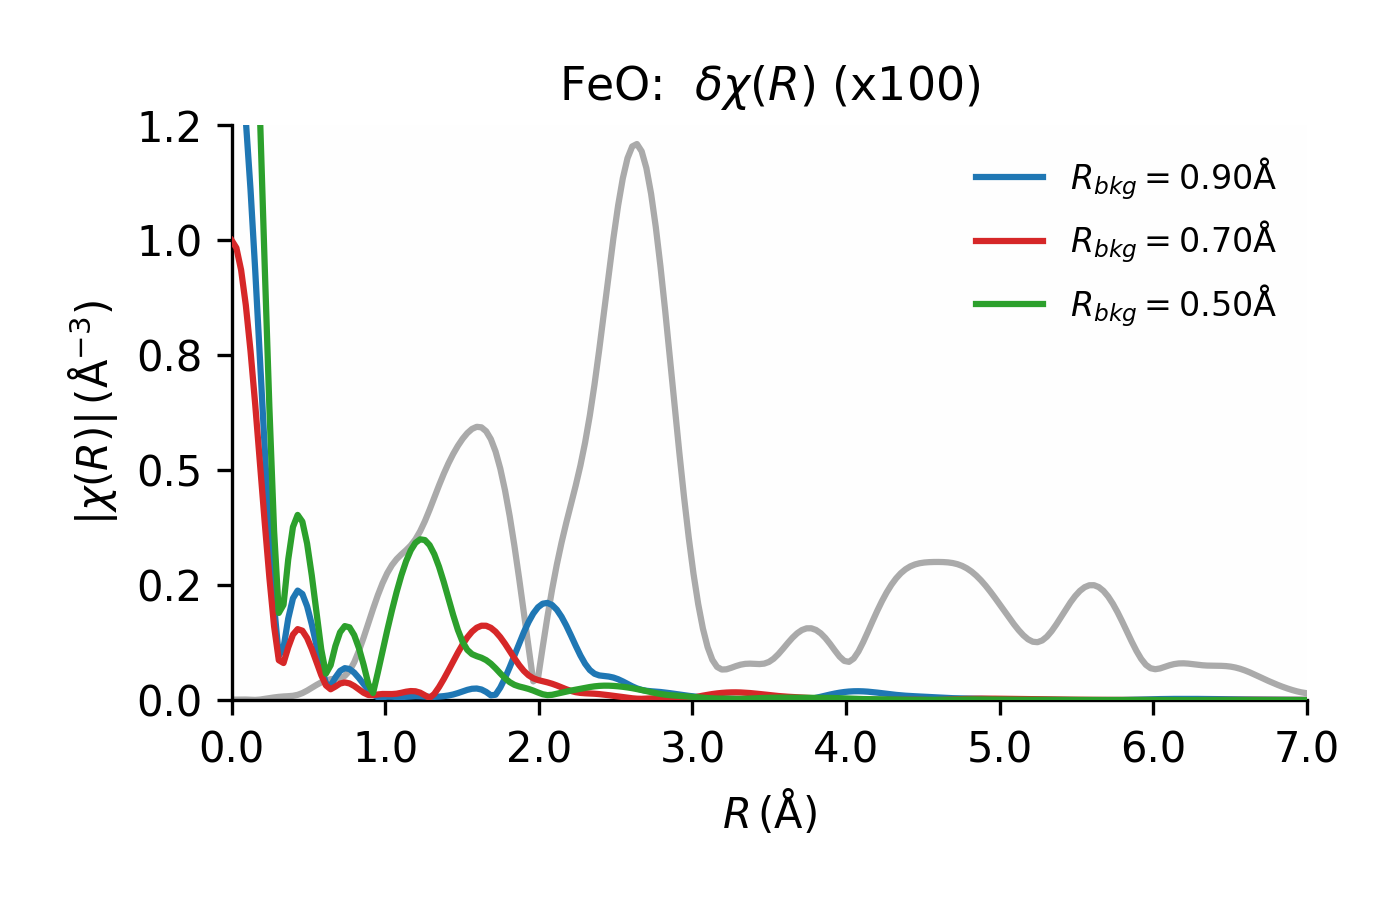
\includegraphics[width=60mm]{figs/errors/feo_deltachir_rbkg} }}

    \end{column}

\end{columns}

\vmm

{\onslide+<3-> {

\begin{cenpage}{105mm}

    Using this $\delta\chi(k)$ array typically reduces the fit $\chi^2$
    statistic by $\sim 3\times$ or even more.

    \vmm

    I think this might need more investigation\ldots

\end{cenpage}

}}


\end{frame}
